% Template latex non officiel pour rapport de TP EEA.
% C'est un template pour thèse que j'ai adapté et 
% auquel j'ai ajouté des éléments au fil du temps pour mes rapports de TP.
% En cas de problèmes n'hésites pas a me contacter.
% David Tocaven
% david.tocaven@gmail.com


%%% /!\ /!\ /!\ /!\ /!\ /!\
% Se compile avec PDFLatex
%%% /!\ /!\ /!\ /!\ /!\ /!\
%%=================================================%%
%%						MAIN
%%=================================================%%


\documentclass[a4paper]{report}

%====================== PACKAGES ======================
\usepackage{bbold}
\usepackage{soul}				% souligner
\usepackage{dsfont}
\usepackage[french]{babel}		% Pour avoir le document en français
\usepackage[utf8x]{inputenc}	% Encodage du document
\usepackage{float}				% Pour gérer les positionnement d'images
\usepackage{amsmath}
\usepackage{mathrsfs}			% Pour les lettres calligraphiques équation
\usepackage[colorinlistoftodos]{todonotes}
\usepackage{url}				% Pour faire des hyperliens vers le web
\usepackage{color}
% pour les informations sur un document compilé en PDF et les liens externes / internes
\usepackage{hyperref}			% Pour faire des hyperliens
\usepackage{array}				% Pour faire des tableaux
\usepackage{tabularx}
% pour utiliser 		% floatbarrier
%\usepackage{placeins}
%\usepackage{floatrow}
\usepackage{setspace}			% Espacement entre les lignes
\usepackage{abstract}			% Modifier la mise en page de l'abstract
\usepackage[T1]{fontenc}		% Police et mise en page (marges) du document
\usepackage[top=2cm, bottom=2cm, left=2cm, right=2cm]{geometry}
\usepackage{pdfpages}			% pour inclures des pdf comme des images
\usepackage{subfig}				% Pour les galerie d'images
\usepackage{listings}			% pour inclure du code dans le doc
\usepackage{soul}				% Pour surligner
\usepackage{enumitem}

\sethlcolor{grisclair}
\definecolor{darkgreen}{RGB}{0,100,0}


%====================== INFORMATION ET REGLES ======================

%rajouter les numérotation pour les \paragraphe et \subparagraphe
\setcounter{secnumdepth}{4}
\setcounter{tocdepth}{4}

\hypersetup{							% Information sur le document
pdfauthor = { NOM },				% Auteurs
pdftitle = {Systèmes Temps Réel},		% Titre du document
pdfsubject = {Compte Rendu de TP},		% Sujet
pdfkeywords = {},				% Mots-clefs
pdfstartview={FitH}}					% ajuste la page à la largueur de l'écran
%pdfcreator = {MikTeX},% Logiciel qui a crée le document
%pdfproducer = {}} % Société avec produit le logiciel

\newcounter{cpt1}						% Compteur pour les n° de ligne dans les prog de l'annexe1
\newcommand\increm{\arabic{cpt1}\addtocounter{cpt1}{1}}
%initialisation de l'intégrateur de language C

%======================= Lstlisting parametres ==================
% Langage C

\lstdefinestyle{customc}{
  breaklines=true,
  frame=L,
  language=C,
  keywordstyle=\bfseries\color{green!40!black},
  commentstyle=\itshape\color{purple!40!black},
  identifierstyle=\color{blue},
  stringstyle=\color{orange},
  tabsize  = 2,
  showstringspaces=false,
}
\lstdefinestyle{customMakefile}{
 language=[gnu] make,
   keywordstyle=\color{teal}\textbf,
   stringstyle=\color{blue},
   identifierstyle=\itshape
   }

\lstdefinestyle{custombash}{
  language=bash,
  basicstyle=\ttfamily
}

%======================== DEBUT DU DOCUMENT ========================

\begin{document}

%\lstset{
%  language=C,                	  % choose the language of the code
%  numbers=left,                   % where to put the line-numbers
%  stepnumber=1,                   % the step between two line-numbers.
%  numbersep=5pt,                  % how far the line-numbers are from the code
%  backgroundcolor=\color{white},  % choose the background color. You must add \usepackage{color}
%  showspaces=false,               % show spaces adding particular underscores
%  showstringspaces=false,         % underline spaces within strings
%  showtabs=false,                 % show tabs within strings adding particular underscores
%  tabsize=2,                      % sets default tabsize to 2 spaces
%  captionpos=b,                   % sets the caption-position to bottom
%  breaklines=true,                % sets automatic line breaking
%  breakatwhitespace=true,         % sets if automatic breaks should only happen at whitespace
%  title=\lstname,                 % show the filename of files included with \lstinputlisting;
%}
%régler l'espacement entre les lignes
\newcommand{\HRule}{\rule{\linewidth}{0.5mm}}


%page de garde
%%=================================================%%
%%						TITRE DU DOCUMENT (1 PAGE)
%							  Pas totalement fini
%%=================================================%%

\begin{titlepage}
\begin{center}

% Upper part of the page. The '~' is needed because only works if a paragraph has started.


\includegraphics[width=0.60\textwidth]{./page_de_garde/logo_ups.png}~\\[1cm]

\textsc{\LARGE Université Paul Sabatier}\\[1.5cm]

\textsc{\Large \bf Systèmes Temps Réel }\\[0.5cm]

% Title
\HRule \\[0.4cm]

{\huge \bfseries  Compte Rendu de TP \textsc{Sujet} -}

\HRule \\[1.5cm]

% Author and supervisor
\begin{minipage}{0.4\textwidth}
\begin{flushleft} \large
\emph{Auteurs: }\\
David \textsc{TOCAVEN}\\
Lucien \textsc{RAKOTOMALALA}\\
\end{flushleft}
\end{minipage}
\begin{minipage}{0.58\textwidth}
\begin{flushright} \large
\emph{Encadrant:} \\
\textbf{ Hamid  \textsc{DEMMOU}}
\end{flushright}
\end{minipage}
\newline
\newline

% une éventuelle image
%\includegraphics[width=.6\textwidth]{./page_de_garde/BACDO_schema.pdf}~\\[1cm]

\vfill
% logo fsi & eea
\begin{tabular}{cc}
   
\includegraphics[height=2cm]{./page_de_garde/logo_fsi.png} \hspace{2cm} &
    \hspace{2cm}
   
\includegraphics[height=2cm]{./page_de_garde/logo_eea.jpg} \\
\end{tabular}

% Bottom of the page
{\large \today}

\end{center}
\end{titlepage}
	

%page blanche
\newpage
~
\tableofcontents
\thispagestyle{empty}
\setcounter{page}{0}
%ne pas numéroter le sommaire


%espacement entre les lignes d'un tableau
\renewcommand{\arraystretch}{1.5}

%====================== INCLUSION DES PARTIES ======================
%
%~
\thispagestyle{empty}
%recommencer la numérotation des pages à "1"
\setcounter{page}{0}

\chapter*{Introduction}
\addcontentsline{toc}{chapter}{Introduction}
\label{chap:Intro}	% Importation de introduction.tex

\chapter{TP 1 : Iniiation a un OS temps Réel basé sur Linux}

\section{Mesures sous linux}
\subsection{Programme $carrelinux-comedi.c$}
Ce premier programme est un générateur de signal carré. Il va nous permettre d'analyser les réponses temps réel de en étant basé sur Linux. Ntre première analyse du programme donne :\begin{itemize}
\item Fonction \emph{Void out} envoie un signal carré. La fréquence semble être défini ailleurs dans le programme. L'amplitude du signal est un niveau logique de \emph{LOW} à \emph{HIGH}.
\item 
\end{itemize}

dans la main est init une structure de temps, est ensuite ouvert la carte entrée sortie.la carte est paramétrée en sortie sur les ports 0 et 1. 
ensuite, l'algorithme attend 
initialisation d'une horloge qui va atenddre un temps correspondant a la demi-période  du signal carré généré


Pou mesurer les modifications de période, nous avons crée deux variables $timespec$ : une qui mesure le temps précédent le sleep, une qui mesure a la fin de l'instance $while(1)$. La mesure de la $\delta$ est : $\delta = t_{debut} - t_{fin}$. 

Mise en place d'un $gnuplot$ pour afficher les 5000 dernières périodes. 

Observation : \begin{itemize}
\item pour aucune charges de linux, les périodes restent à $50\mu s$. 
\item pour un simple 
\end{itemize}

\section{Mesures sous RTAI}

Utilisation de la ligne : 




\chapter{Conception d'un logiciel Temps réel}

\section{Mesures sous Linux}
\subsection{Programme $carrelinux-comedi.c$}
Ce premier programme est un générateur de signal carré. Il va nous permettre d'analyser les réponses temps réel de en étant basé sur Linux. Notre première analyse du programme donne :\begin{itemize}
\item Fonction \emph{Void out} : envoie un signal inverse  celui qu'elle envoyait précédemment. La fréquence semble être défini ailleurs dans le programme. Le signal est envoyé vers le port 0 de la carte E/S initialisé dans la fonction \emph{main}.
\item \emph{Carte E/S} : la librairie $Comedio$ permet d'ouvrir la connexion série avec la carte d'entrée sortie puis d'initialiser le sens du port.
\item \emph{main} : Initialisation d'une structure de temps dans le main qui sera utilisé dans la boucle infinie du programme principal.
\end{itemize}
Le programme entre ensuite dans une boucle infinie dans laquelle il attend un temps \emph{TIMER\_ABSTIME} pour ensuite appeler la fonction \emph{out}. Après, le programme calcule le \emph{next shot}, i.e le prochain déclenchement, qu'il devra attendre lors du recommencement de la boucle.

Avec ce recueil d'informations, nous sommes capable de définir la fréquence du signal du signal carré que nous allons observer : elle est égale à 2 fois le \emph{next shot} calculé dans la boucle infinie : ce calcul est : $next\_shot = 50 000 + t$, la variable $t$ appartient à la structure de temps et elle est défini en nanosecondes donc : \begin{equation}
f = 2\times 50 000ns \Leftrightarrow f= 100\mu s
\end{equation} 

\subsection{Mesures des période du signal}
Pour mesurer les modifications de période, nous avons crée deux variables de type $timespec$ : une qui mesure le temps précédent le sleep, une qui mesure a la fin de l'instance $while(1)$. La mesure de la demi-période du signal carré $\delta$ est alors la différence entre le temps du début de la boucle et le temps en fin de boucle.  

Pour permettre un affichage correct, nous avons introduit dans notre programme une fonction qui permet d'écrire dans un fichier les 5000 dernières $\delta$ mesurées et qui sera appelé dès que le signal \textbf{Ctrl+C} grâce à l'instruction : 
\begin{lstlisting}[style = customc]
signal(SIGINT, IntHandler)
\end{lstlisting} 
Nous utilisons ensuite le fichier de mesure en .res pour un affiche avec un script $gnuplot$. Nous observons les résultats suivants :
\begin{center}
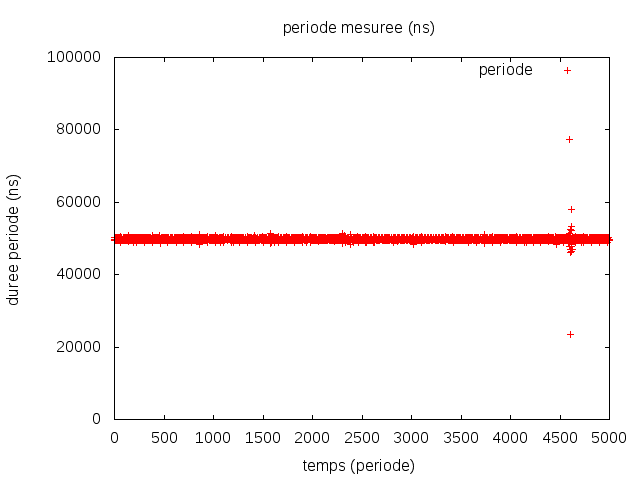
\includegraphics[width = .8\textwidth]{./I/images/delta_no_perturb.png}
\captionof{figure}{Mesure des périodes sans perturbation}
\end{center}

Pour cette première observation, nous n'avons pas touché le système d'exploitation pendant la mesure des périodes et cependant, nous remarquons que celles ci ont eu out de même quelques légères perturbations. Nous allons maintenant effectué quelques perturbations pendant que le relevé s'effectue. 

\begin{center}
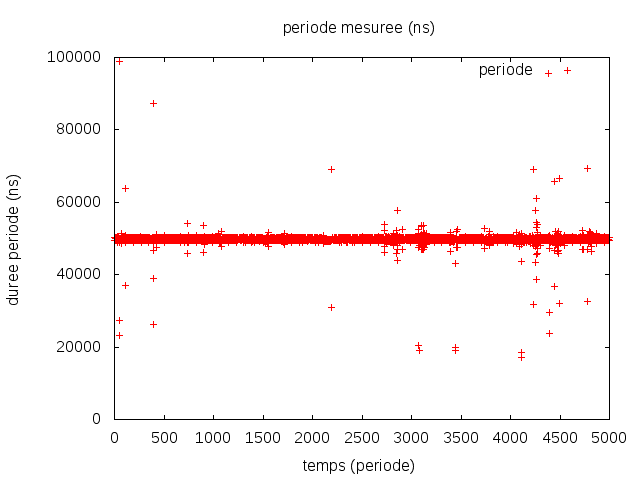
\includegraphics[width = \textwidth]{./I/images/delta1.png}
\captionof{figure}{Mesures des périodes avec quelques perturbations}
\end{center}
Nous notons ici que les petites perturbations commencent à avoir de grosse conséquence sur la demi période du signal. Ces perturbations se notent aussi sur l'oscilloscope où nous observons des modifications du signal. Pour terminer cette étude, nous effectuons une dernière mesure des périodes dans laquelle nous demandons au système d'exploitation une concaténation de fichier volumineux. 


\begin{center}
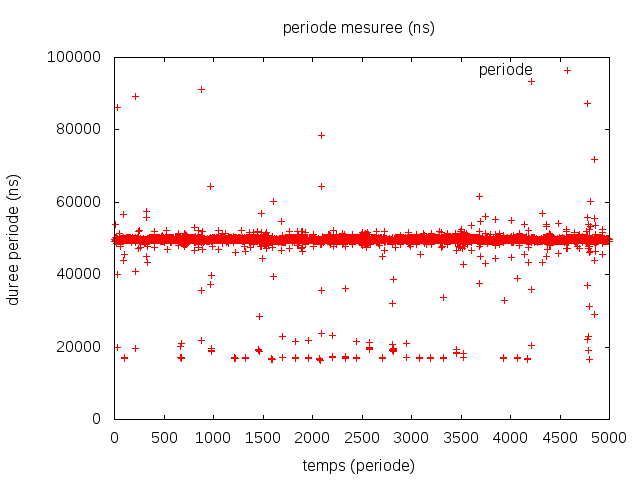
\includegraphics[width = \textwidth]{./I/images/delta_cat.png}
\captionof{figure}{Mesures des périodes avec la commande "cat /dev/zer > file2delete" en parallèle}
\end{center}

Nous observons que la dispersion des périodes est beaucoup plus importante. Le système d'exploitation n'a pas réussi à ordonnancer notre programme avec l'instruction que nous lui avons demandé. De telles différences ne sont pas acceptables pour des applications ou des systèmes Temps Réel. Le système d'exploitation Linux seul ne peut pas être utilisé tel quel pour le Temps réel, nous devons ajouter au noyau la capacité à préempter des tâches avec l'architecture logicielle RTAI.
\section{2 }	


\chapter{}

%\chapter{}



%\input{./V/chap5.tex}

%\input{./VI/chap6.tex}

%\input{./conclusions/conclusions.tex}

\chapter{Conclusion}

%Ne pas numéroter cette partie
\part*{Annexes}
%Rajouter la ligne "Annexes" dans le sommaire
\addcontentsline{toc}{part}{Annexes}

\chapter*{Annexe 1 - TP 1}
\addcontentsline{toc}{chapter}{TP1}
\section{Mesures sous Linux}
\subsection{Programme $carrelinux-comedi.c$}
Ce premier programme est un générateur de signal carré. Il va nous permettre d'analyser les réponses temps réel de en étant basé sur Linux. Notre première analyse du programme donne :\begin{itemize}
\item Fonction \emph{Void out} : envoie un signal inverse  celui qu'elle envoyait précédemment. La fréquence semble être défini ailleurs dans le programme. Le signal est envoyé vers le port 0 de la carte E/S initialisé dans la fonction \emph{main}.
\item \emph{Carte E/S} : la librairie $Comedio$ permet d'ouvrir la connexion série avec la carte d'entrée sortie puis d'initialiser le sens du port.
\item \emph{main} : Initialisation d'une structure de temps dans le main qui sera utilisé dans la boucle infinie du programme principal.
\end{itemize}
Le programme entre ensuite dans une boucle infinie dans laquelle il attend un temps \emph{TIMER\_ABSTIME} pour ensuite appeler la fonction \emph{out}. Après, le programme calcule le \emph{next shot}, i.e le prochain déclenchement, qu'il devra attendre lors du recommencement de la boucle.

Avec ce recueil d'informations, nous sommes capable de définir la fréquence du signal du signal carré que nous allons observer : elle est égale à 2 fois le \emph{next shot} calculé dans la boucle infinie : ce calcul est : $next\_shot = 50 000 + t$, la variable $t$ appartient à la structure de temps et elle est défini en nanosecondes donc : \begin{equation}
f = 2\times 50 000ns \Leftrightarrow f= 100\mu s
\end{equation} 

\subsection{Mesures des période du signal}
Pour mesurer les modifications de période, nous avons crée deux variables de type $timespec$ : une qui mesure le temps précédent le sleep, une qui mesure a la fin de l'instance $while(1)$. La mesure de la demi-période du signal carré $\delta$ est alors la différence entre le temps du début de la boucle et le temps en fin de boucle.  

Pour permettre un affichage correct, nous avons introduit dans notre programme une fonction qui permet d'écrire dans un fichier les 5000 dernières $\delta$ mesurées et qui sera appelé dès que le signal \textbf{Ctrl+C} grâce à l'instruction : 
\begin{lstlisting}[style = customc]
signal(SIGINT, IntHandler)
\end{lstlisting} 
Nous utilisons ensuite le fichier de mesure en .res pour un affiche avec un script $gnuplot$. Nous observons les résultats suivants :
\begin{center}
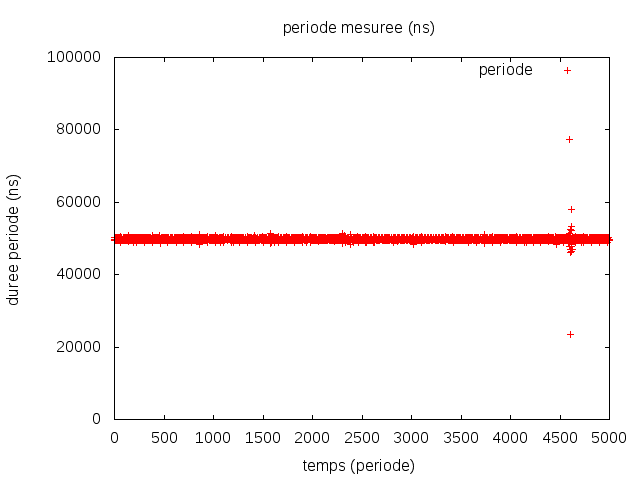
\includegraphics[width = .8\textwidth]{./I/images/delta_no_perturb.png}
\captionof{figure}{Mesure des périodes sans perturbation}
\end{center}

Pour cette première observation, nous n'avons pas touché le système d'exploitation pendant la mesure des périodes et cependant, nous remarquons que celles ci ont eu out de même quelques légères perturbations. Nous allons maintenant effectué quelques perturbations pendant que le relevé s'effectue. 

\begin{center}
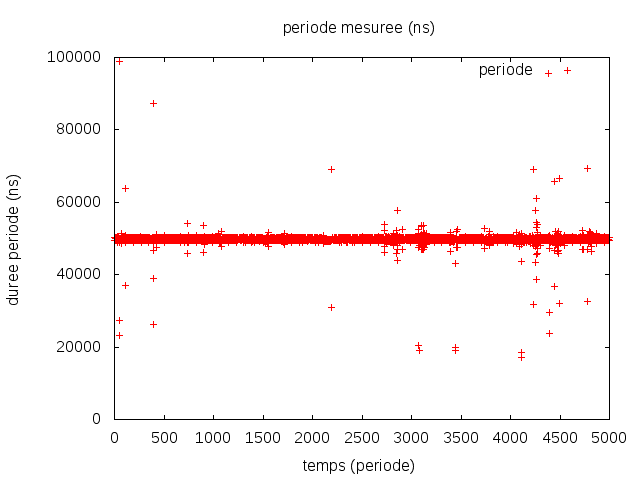
\includegraphics[width = \textwidth]{./I/images/delta1.png}
\captionof{figure}{Mesures des périodes avec quelques perturbations}
\end{center}
Nous notons ici que les petites perturbations commencent à avoir de grosse conséquence sur la demi période du signal. Ces perturbations se notent aussi sur l'oscilloscope où nous observons des modifications du signal. Pour terminer cette étude, nous effectuons une dernière mesure des périodes dans laquelle nous demandons au système d'exploitation une concaténation de fichier volumineux. 


\begin{center}
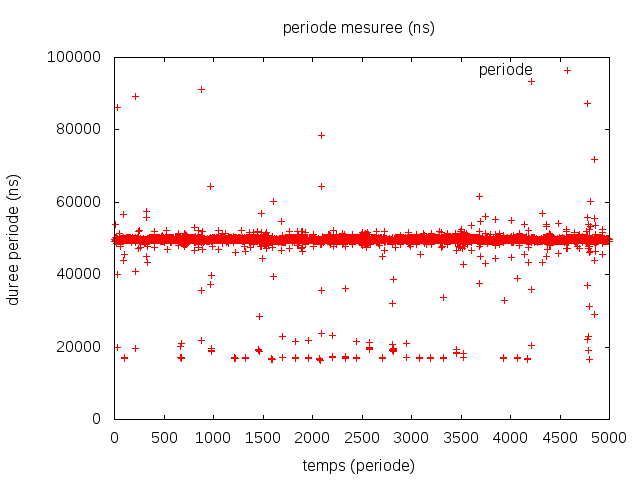
\includegraphics[width = \textwidth]{./I/images/delta_cat.png}
\captionof{figure}{Mesures des périodes avec la commande "cat /dev/zer > file2delete" en parallèle}
\end{center}

Nous observons que la dispersion des périodes est beaucoup plus importante. Le système d'exploitation n'a pas réussi à ordonnancer notre programme avec l'instruction que nous lui avons demandé. De telles différences ne sont pas acceptables pour des applications ou des systèmes Temps Réel. Le système d'exploitation Linux seul ne peut pas être utilisé tel quel pour le Temps réel, nous devons ajouter au noyau la capacité à préempter des tâches avec l'architecture logicielle RTAI.
\newpage
\section{2 }	


\chapter*{Annexe 2 - TP 2}

\addcontentsline{toc}{chapter}{Annexe 2 - TP2}
\setcounter{section}{0}
\setcounter{subsection}{0}

\subsection*{Code source du TP 2 \textbf{tp2\_gen\_sign}}
\lstinputlisting[style=customc]{./annexes/annexe2/tp2_gen_sign.c}
% **********************************
	%


\newpage

%récupérer les citation avec "/footnotemark"
\nocite{*}

%%choix du style de la biblio
%\bibliographystyle{unsrt}
%%inclusion de la biblio
%\bibliography{bibliographie}
%%voir wiki pour plus d'information sur la syntaxe des entrées d'une bibliographie

\end{document}

